\section{Texture mapping}

\subsection{Linear Texture mapping}
The problem solved in this section can be described as follows:
\newline
Given two images, one of a texture and one of a plane, the texture is
mapped onto the plane. 

\begin{figure}[H]
    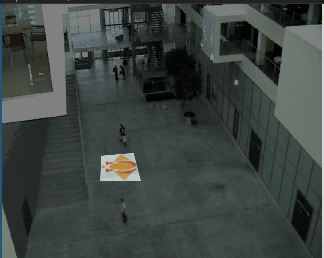
\includegraphics{pics/mapping.png}
    \label{mapping}
\end{figure}

The steps to achieve this are few. 

First, a homography is obtained between the two images though 4 points in each.
These can be selected by the user, or the corners of the image can be used
for the texture. This homography is used to perform a perspective
transform on the texture image with the dimensions of the destination
image. This "warped" image is then used as an overlay on the destination
image. To apply this "overlay" we calculate the weighted sum of the two
arrays (images), the result of this operation is the result image

\subsubsection{Code}
We leverage cv2 to do most of the work here

\begin{verbatim}
    # Grab the homography
    H,Points  = SIGBTools.getHomographyFromMouse(I1,I2,4)
    
    # Dimensions
    h,w,d = I2.shape

    #Perspective transformation
    overlay = cv2.warpPerspective(I1, H,(w, h))

    # Weigthed sum
    M = cv2.addWeighted(I2, 0.5, overlay, 0.5,0)
    
    # Show the image
    cv2.imshow("Overlayed Image",M)

\end{verbatim}

\subsection{Realistic texture mapping}

The problem solved in this section can be described as follows:
\newline
Given two images, one of a texture and one of a plane, the texture is
mapped onto the plane with a single click in the destination image and with
preservation of the textures original dimensions

This problem will be solved through the use of forward mapping and two
homographies.

To do it we use 3 parameters.

First we "cheat" beforehand by using a previously obtained homography. This
Homography is saved when we map the ground view to the map, as described in
a previous section. It goes between the map and ground floor images. This homography determines our mapping, and as such
dictates the quality of the result, and is one our inputs.
The second is a user selected point, determining where the center of the
texture will be placed. Lastly, we modify the texture with scaling
parameter.

Using the obtained homography we can determine where the texture will be
placed in the destination image. We need a center of the texture
destination, and the aspect ratio of the texture. Using this we can
determine the position of the 4 points of the texture. 

To get the center, we simply apply our homography to the clicked point in the
original image, giving us the point in the destination image. To find the four
projected points for the texture we use the corners of the image in the
original texture. Between these four points we need to estimate a
homography to four corresponding points in the destination image. These four
points are obtained by using the projected selected point as origin and select
four corners with a distance of the same aspect ratio as in the original image.
With this homography we can create a transformation matrix consisting of the
identity matrix with only the translation components changed,
effectively lettings us "move" the texture to the correct points. Since we
also want to scale the texture (according to our provided scale
parameter) we will also affect the scaling parameters of the matrix to
"stretch" the texture. Lastly, we do as in the previous section.
Calculate a projection matrix and apply by calculating the weighted sum of the
the original image and the warped texture.


